\documentclass{article}
    % General document formatting
    \usepackage[margin=0.7in]{geometry}
    \usepackage[parfill]{parskip}
    \usepackage[utf8]{inputenc}
    \usepackage{amsmath}
    \usepackage{amssymb}
    \usepackage{tikz}
    \usepackage{fancyhdr}
    \usepackage{listings}
    \usepackage{multicol}
    \usepackage{polynom}

\pagestyle{fancy}
\fancyhf{}
\rhead{Edgar Jacob Rivera Rios - A01184125}

\begin{document}
\begin{titlepage}

    \newcommand{\HRule}{\rule{\linewidth}{0.5mm}} % Defines a new command for the horizontal lines, change thickness here

    \center % Center everything on the page

    %----------------------------------------------------------------------------------------
    %	HEADING SECTIONS
    %----------------------------------------------------------------------------------------

    \textsc{\LARGE Tecnológico de Monterrey}\\[1.5cm] % Name of your university/college
    \textsc{\Large Fundamentos de computación}\\[0.5cm] % Major heading such as course name
    %\textsc{\large Minor Heading}\\[0.5cm] % Minor heading such as course title

    %----------------------------------------------------------------------------------------
    %	TITLE SECTION
    %----------------------------------------------------------------------------------------

    \HRule \\[0.4cm]
    { \huge \bfseries Homework 9}\\[0.4cm] % Title of your document
    \HRule \\[1.5cm]

    %----------------------------------------------------------------------------------------
    %	AUTHOR SECTION
    %----------------------------------------------------------------------------------------

    \begin{minipage}{0.4\textwidth}
    \begin{flushleft} \large
    \emph{Student:}\\
    Jacob \textsc{Rivera} % Your name
    \end{flushleft}
    \end{minipage}
    ~
    \begin{minipage}{0.4\textwidth}
    \begin{flushright} \large
    \emph{Professor:} \\
    Dr. Hugo \textsc{Terashima} % Supervisor's Name
    \end{flushright}
    \end{minipage}\\[2cm]

    % If you don't want a supervisor, uncomment the two lines below and remove the section above
    %\Large \emph{Author:}\\
    %John \textsc{Smith}\\[3cm] % Your name

    %----------------------------------------------------------------------------------------
    %	DATE SECTION
    %----------------------------------------------------------------------------------------

    {\large \today}\\[2cm] % Date, change the \today to a set date if you want to be precise

    %----------------------------------------------------------------------------------------
    %	LOGO SECTION
    %----------------------------------------------------------------------------------------

    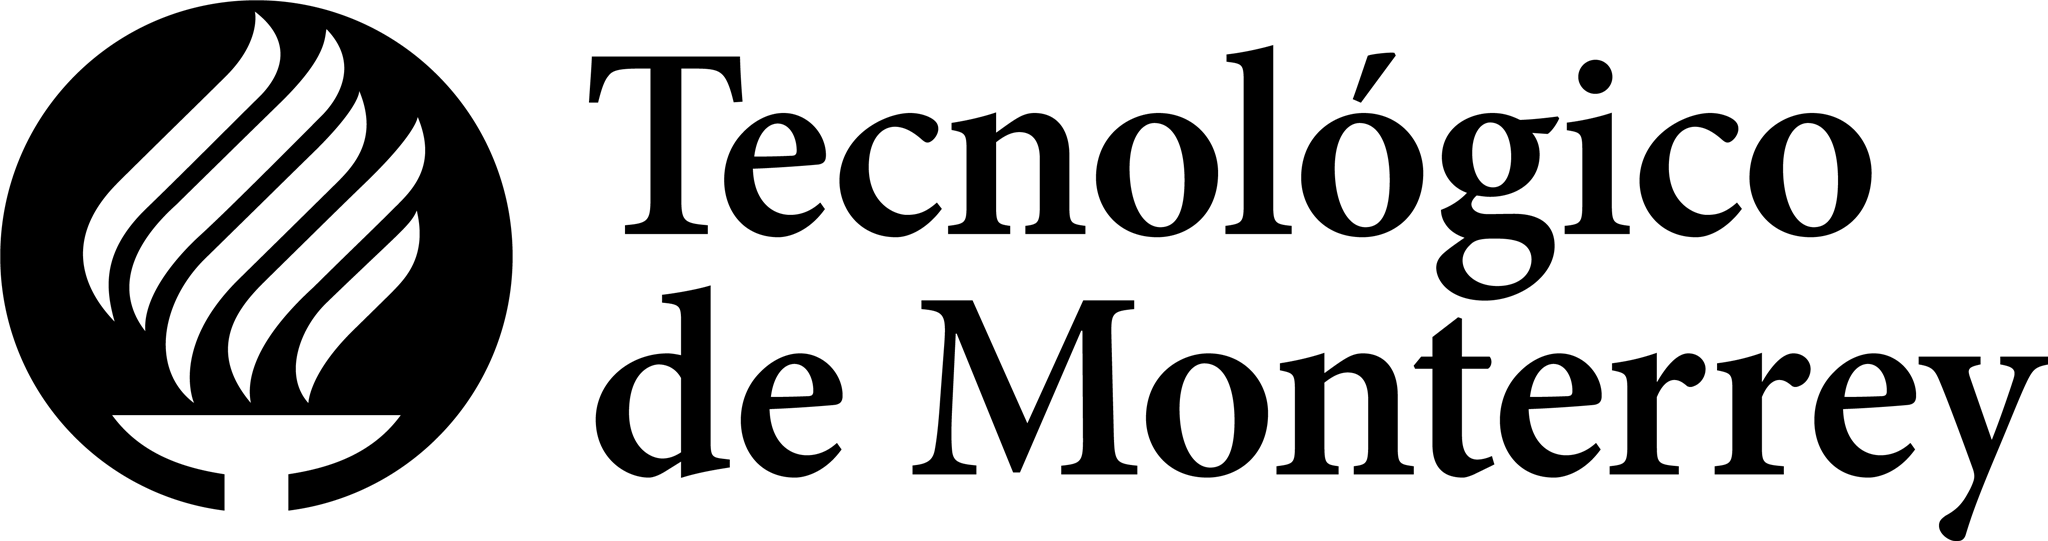
\includegraphics[width=0.4\textwidth,height=\textheight,keepaspectratio]{logo-tec-negro.png} % Include a department/university logo - this will require the graphicx package

    %----------------------------------------------------------------------------------------

    \vfill % Fill the rest of the page with whitespace

\end{titlepage}


\section{Problems}
Solve the following problems:
\begin{enumerate}
    \item What is a P problem?

    A problem that can be solved in polynomial time

    \item What is an NP problem?

    A problem which result can be verified in polynomial time, but has a non-deterministic solution time.

    \item What is and NP - complete problem?

    This are the problems that are at least as hard as the hardest NP problems. This means, the ones that are both NP and NP-Hard.

    \item Why P = NP is considered an open problem?

    It is the question that arises from comparing P and NP problems, it is known that P is included in NP, but we do not know if the NP problems can be reduced to be solved in P time, making P and NP the same.
    It is currently considered an open problem there is not a mathematical proof that NP is equal or different to P.

    \item What is the difference between a decision problem and an optimization problem?

    A decision problem returns as result a simple $yes$, $no$ answer, and a optimization problem tries to find the best values for certain defined parameters.

    \item Investigate the 2-dimensional packing problem, describe the problem, and state it as a decision problem and then as an optimization problem?

    In the problem, you are presented with a series of items with different dimensions and bins of fixed dimensions, the objective is to fit the items in as few bins as possible.

    As a decision problem:\\
    Is it possible to fit the items in $n$ bins?

    As a optimization problem:\\
    Find the combinations of items which fit in the least amount of bins possible

    \item Describe a simple heuristic (approximation algorithm) for solving the 2-dimensional packing problem. How could you measure the effectiveness of this heuristic for solving the problem?

    The characterization of the items can be used to solve the problem, you could use the average of width and height to decide if it's better to fill a bin as much as possible or open a new one. The quantity of bins is definitive measure to use when testing the heuristic.

    \item Can you describe the Travelling Salesman Problem? How is this problem related to the Hamiltonian Cycle? Provide a polynomial transformation between those problems. How are these problems related
    to the Vehicle Routing Problem?

    The traveling salesman problem is a problem which states that given a list of cities and the distances between them, to return the shortest path that visits each city and returns to the initial city. This is basically a specialization of the problem of the Hamiltonian circle, which consists on finding a cycle which given a graph, tries to get a cycle which passes for each node once. The vehicle routing problem is a generalization of the the Traveling Salesman Problem.

    \item What is a phase transition?
    
    It is a transformation for the inputs from one problem to another

    \item How is a phase transition related to the easiness or hardness of NP problems?

    By using a phase transition, you can either simplify or maker harder the problem by converting in another problem. For example, you can use a phase transition to convert an NP problem to an NP-Hard problem

\end{enumerate}
\end{document}